\documentclass[conference,a4paper]{IEEEtran}
\usepackage{fontspec}
\usepackage{polyglossia}
\setdefaultlanguage[variant=brazilian]{portuguese}
\emergencystretch=2em \hyphenpenalty=50
\usepackage{graphicx,booktabs,array,tabularx,tikz,xcolor,hyperref,enumitem,caption}
\usetikzlibrary{arrows.meta,positioning,shapes.misc,calc,fit}
\hypersetup{colorlinks,linkcolor=black,citecolor=black,urlcolor=blue!50!black,breaklinks}
\setmainfont{TeX Gyre Termes}
\setmonofont{DejaVu Sans Mono}[Scale=0.85]
\captionsetup{font=small,labelfont=bf}
\newcolumntype{Y}{>{\raggedright\arraybackslash}X}
\newcommand{\code}[1]{\texttt{#1}}
\definecolor{resp}{HTML}{0284C7}\definecolor{hr}{HTML}{E11D48}\definecolor{boxbg}{HTML}{F3F4F6}

\begin{document}
\title{Estetoscópio digital experimental com ESP32-C3 e aplicativo web via Web Bluetooth:\\ documentação técnica do aplicativo e especificação de interface com o firmware}

\author{\IEEEauthorblockN{Davi Braga Padilha Azevedo}
\IEEEauthorblockA{Engenharia Elétrica — Universidade Federal de Minas Gerais\\
Repositório: \url{https://github.com/DaviAzvd/estetoscopio-esp32} \quad Aplicativo: \url{https://daviazvd.github.io/estetoscopio-esp32/}\\
Versão do documento: 5 de novembro de 2026 (commit \code{89f930f})}}
\maketitle

\begin{abstract}
Este documento descreve o aplicativo de visualização e análise de sons de ausculta (respiratória e cardíaca) desenvolvido para o projeto de disciplina de um estetoscópio digital baseado no microcontrolador ESP32-C3 Super Mini. Justifica-se a escolha de uma página web executada no Chrome para Android, com a API Web Bluetooth, em lugar de um aplicativo nativo; descreve-se a arquitetura, na qual o microcontrolador apenas amostra o conversor A/D e transmite os valores crus por Bluetooth Low Energy (BLE), ficando toda a filtragem e análise no aplicativo; apresentam-se as duas telas de operação e os resultados esperados; documentam-se a origem, a licença e os valores de referência das gravações reais usadas na simulação; e especifica-se, em uma seção autocontida, o contrato de interface que o firmware deve cumprir. Encerra-se com a lista de pontos ainda não definidos. Todas as afirmações técnicas trazem referência às fontes. O projeto é acadêmico; o sistema não é dispositivo médico e não se destina a diagnóstico.
\end{abstract}

\section{O que é}
O sistema captura, por um microfone acoplado ao tórax, os sons de ausculta de uma pessoa e os apresenta em tempo real em um tablet ou telefone Android: forma de onda (fonocardiograma), envelope de intensidade, espectrograma, frequência respiratória ou cardíaca e indicadores derivados (razão inspiração/expiração e regularidade do ritmo). O hardware é um ESP32-C3 Super Mini com um estágio analógico de condicionamento (amplificador, filtro passa-alta e passa-baixa, 20--1000~Hz) e um conversor A/D (ADC). O aplicativo é um único arquivo HTML, publicado em GitHub Pages, que se conecta ao ESP32-C3 por BLE diretamente do navegador.

Princípio de projeto adotado após discussão da equipe: \emph{o ESP32-C3 faz o mínimo}. Ele amostra o ADC a uma taxa fixa e envia os valores crus; nenhum filtro, nenhum cálculo e nenhum ``modo'' existem no firmware. Isso concentra toda a complexidade de processamento de sinal no aplicativo, onde é mais fácil de desenvolver, depurar e alterar, e deixa o firmware livre para cuidar de LED, bateria e alimentação.

\section{Por que uma página web, e não um aplicativo Android nativo}
\label{sec:web}
A alternativa óbvia seria um aplicativo Android (Android Studio/Kotlin ou Flutter). A escolha pela página web foi deliberada, pelos motivos abaixo.

\begin{enumerate}[leftmargin=*]
\item \textbf{Capacidade técnica suficiente.} A API Web Bluetooth permite a páginas web, no papel de \emph{central}, conectar-se a servidores GATT por BLE, assinar notificações de características e detectar desconexões~\cite{chrome-wb}. É exatamente o que o projeto requer.
\item \textbf{Sem cadeia de ferramentas.} Não há SDK, compilação, assinatura de pacote nem loja de aplicativos. O aplicativo é um arquivo \code{index.html}; qualquer alteração entra em produção com um \code{git push}, porque o repositório publica automaticamente em GitHub Pages por uma ação de CI.
\item \textbf{Instalação trivial em qualquer Android.} Basta abrir a URL no Chrome e usar ``Adicionar à tela inicial''. O manifesto de aplicativo web faz a página abrir em tela cheia, com ícone próprio, como um aplicativo.
\item \textbf{Funciona offline depois da primeira abertura.} Um \emph{service worker} guarda em cache a página e as gravações de simulação; o Bluetooth não depende de internet. (Ver Seção~\ref{sec:oper}.)
\item \textbf{Depuração no PC.} A mesma página roda no Chrome de desktop, o que permitiu validar todo o pipeline de sinal com gravações reais antes de o hardware existir (Seção~\ref{sec:sim}).
\end{enumerate}

\noindent\textbf{Limitações aceitas.} A Web Bluetooth é uma API de disponibilidade limitada: está disponível no Chrome, Edge, Opera e Samsung Internet, mas não no Firefox nem no Safari (iOS)~\cite{mdn-wb}. Portanto, iPhones e iPads ficam fora do escopo; para o trabalho, o alvo é um tablet Android, o que é suficiente. A API exige \emph{contexto seguro} (HTTPS) e um gesto do usuário para iniciar a busca de dispositivos~\cite{mdn-wb,chrome-wb}; GitHub Pages serve os sites sempre por HTTPS~\cite{gh-pages-https}, o que resolve o primeiro requisito, e o botão ``Conectar BLE'' resolve o segundo.

\section{Arquitetura e funcionamento}
\subsection{Visão geral}
A Fig.~\ref{fig:arq} resume a cadeia de sinal. À esquerda, o hardware; à direita, o aplicativo. A fronteira entre os dois é o enlace BLE, cujo contrato está na Seção~\ref{sec:esp}.

\begin{figure}[t]
\centering
\begin{tikzpicture}[font=\scriptsize,node distance=3mm and 3mm,
 box/.style={draw,rounded corners=2pt,minimum height=7mm,align=center,inner sep=2pt,fill=boxbg},
 hw/.style={box,fill=hr!8},sw/.style={box,fill=resp!8},
 arr/.style={-{Latex[length=2mm]},thick}]
\node[hw,minimum width=13mm] (mic) {Microfone};
\node[hw,right=of mic,minimum width=14mm] (amp) {Amp.\\+ filtros\\20--1000 Hz};
\node[hw,right=of amp,minimum width=15mm] (adc) {ESP32-C3\\ADC 12 bit\\4 kHz};
\node[hw,right=of adc,minimum width=13mm] (ble) {BLE\\notify\\242 B};
\draw[arr] (mic)--(amp); \draw[arr] (amp)--(adc); \draw[arr] (adc)--(ble);
\node[sw,below=6mm of ble,minimum width=15mm] (wb) {Chrome\\Web Bluetooth};
\node[sw,left=of wb,minimum width=16mm] (dsp) {Filtros IIR\\por modo\\RMS 50 Hz};
\node[sw,left=of dsp,minimum width=17mm] (ana) {Detecção\\FR / FC\\I:E, regular.};
\node[sw,left=of ana,minimum width=14mm] (ui) {Telas\\gráficos\\CSV/WAV};
\draw[arr] (ble)--node[right]{\tiny 33 pkt/s}(wb); \draw[arr] (wb)--(dsp); \draw[arr] (dsp)--(ana); \draw[arr] (ana)--(ui);
\node[draw,dashed,fit=(mic)(ble),inner sep=3pt,label={[anchor=south west,font=\tiny,yshift=-1pt]north west:hardware (eletrônica + firmware)}] {};
\node[draw,dashed,fit=(wb)(ui),inner sep=3pt,label={[anchor=north west,font=\tiny,yshift=1pt]south west:aplicativo web (este documento)}] {};
\end{tikzpicture}
\caption{Cadeia de sinal. O ESP32-C3 não filtra nem calcula: envia amostras cruas do ADC. Todo o processamento ocorre no navegador.}
\label{fig:arq}
\end{figure}

\subsection{Processamento no aplicativo}
Cada amostra recebida (inteiro 0--4095) tem o nível médio removido (2048) e passa por:
\begin{itemize}[leftmargin=*]
\item \textbf{Filtro passa-faixa do modo} (Butterworth de 4\textsuperscript{a} ordem, dois biquads passa-alta e dois passa-baixa, coeficientes RBJ recalculados para a taxa escolhida): 100--1000~Hz em \emph{Respiração}, 20--150~Hz em \emph{Batimento}. As bandas vêm da literatura: o som vesicular normal ocupa 100--1000~Hz, com queda de potência acima de \textasciitilde200~Hz, e sibilos têm energia em 100--1000~Hz~\cite{bohadana2014,kim2023}; a energia de B1 e B2 concentra-se abaixo de 150~Hz~\cite{arnott1984}.
\item \textbf{Envelope RMS} em janelas de 20~ms (50 valores/s), que alimenta o gráfico de envelope e os detectores.
\item \textbf{Frequência respiratória}: detecção de picos do envelope com limiar adaptativo e período refratário de 2,5~s; a razão I:E é estimada pelos tempos acima/abaixo do limiar (aproximação; ver Seção~\ref{sec:aberto}).
\item \textbf{Frequência cardíaca}: autocorrelação do envelope em janela de 10~s, buscando o período entre 0,4 e 1,5~s (40--150~bpm), com mediana das cinco últimas estimativas. A autocorrelação foi adotada porque um detector de picos simples contava B1 e B2 como batimentos distintos (lia 180~bpm em uma gravação de 61~bpm). A ``regularidade'' exibida é a altura normalizada do pico de autocorrelação.
\item \textbf{Espectrograma} do sinal bruto (FFT de 512 pontos, passo 256), até metade da taxa de amostragem, com as bordas da banda do modo sobrepostas.
\end{itemize}
Além disso, o aplicativo contabiliza pacotes recebidos e perdidos (pelo contador de sequência), amostras por segundo (comparadas à taxa esperada), o valor instantâneo do ADC e o número de amostras saturadas (0 ou 4095). Esses quatro números são o instrumento de validação do hardware sem osciloscópio.

\section{As telas e o resultado esperado}
O aplicativo tem uma única página com dois modos, selecionados no topo; o modo muda o filtro, os indicadores, a cor de destaque e os pontos de ausculta do diagrama. As Figs.~\ref{fig:resp} e \ref{fig:hr} mostram as duas telas em simulação (Seção~\ref{sec:sim}); a Fig.~\ref{fig:dlg} mostra o pop-up de medição.

\begin{figure*}[t]
\centering
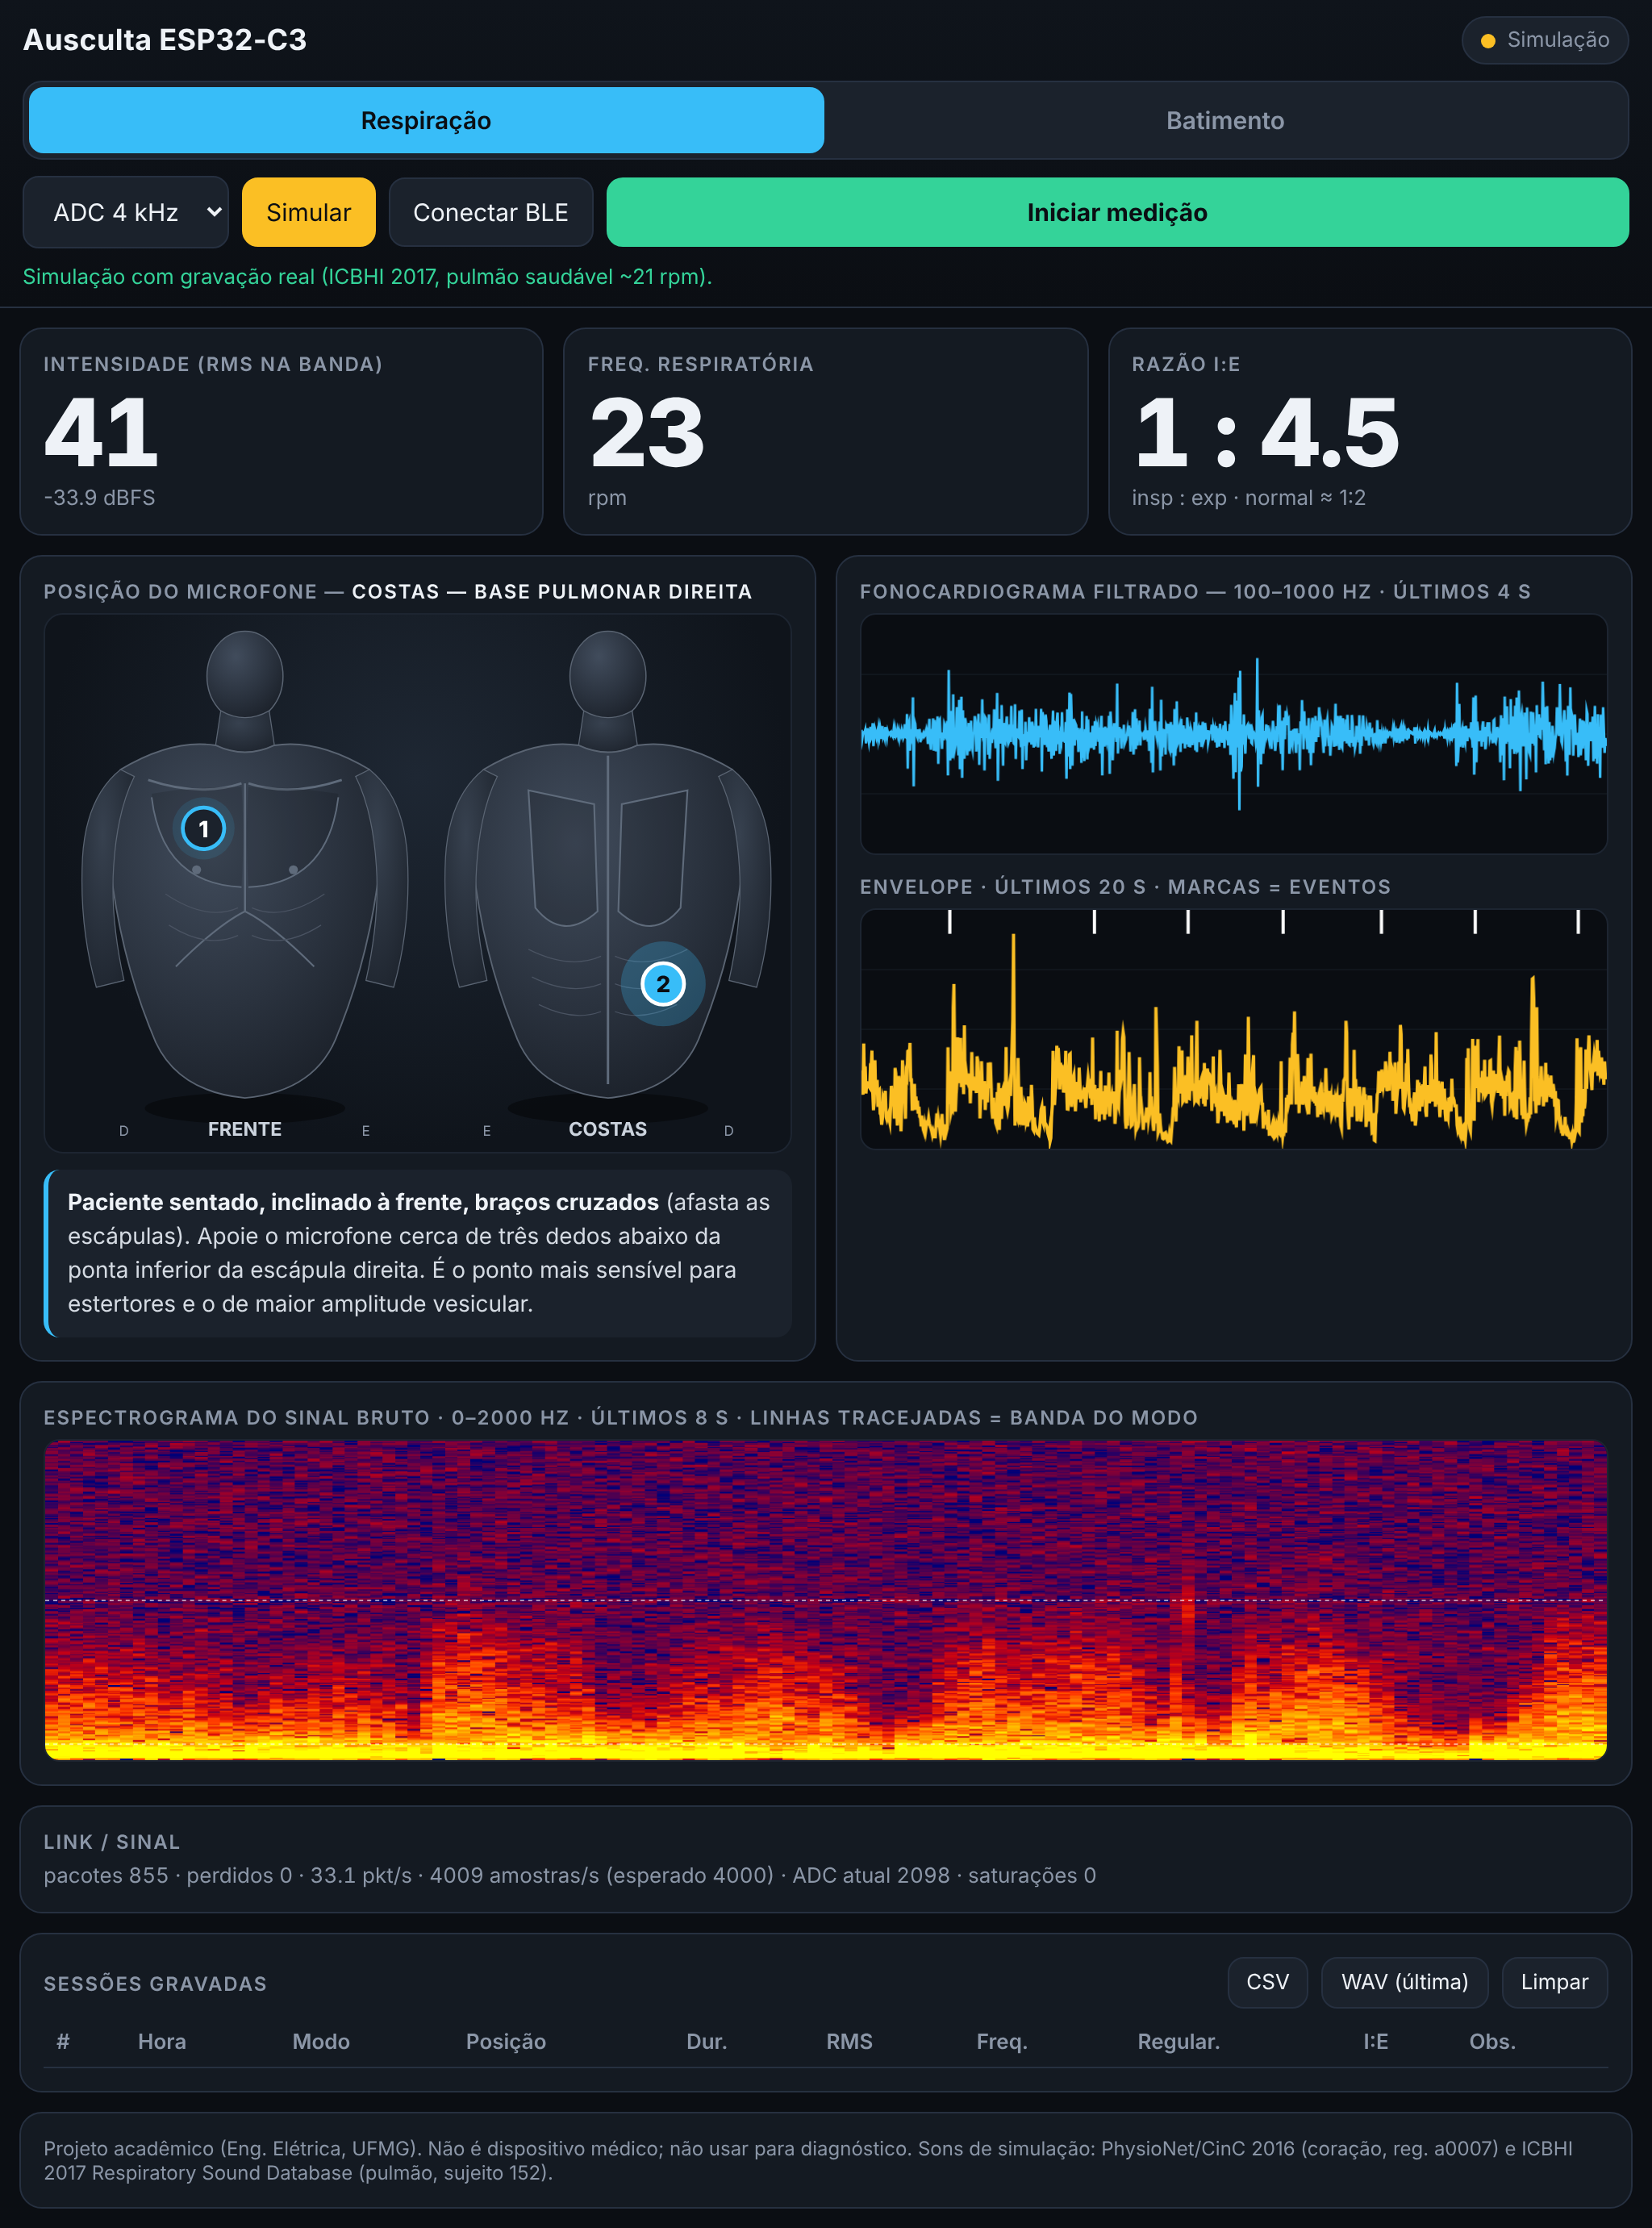
\includegraphics[width=0.49\textwidth]{fig_resp.png}\hfill
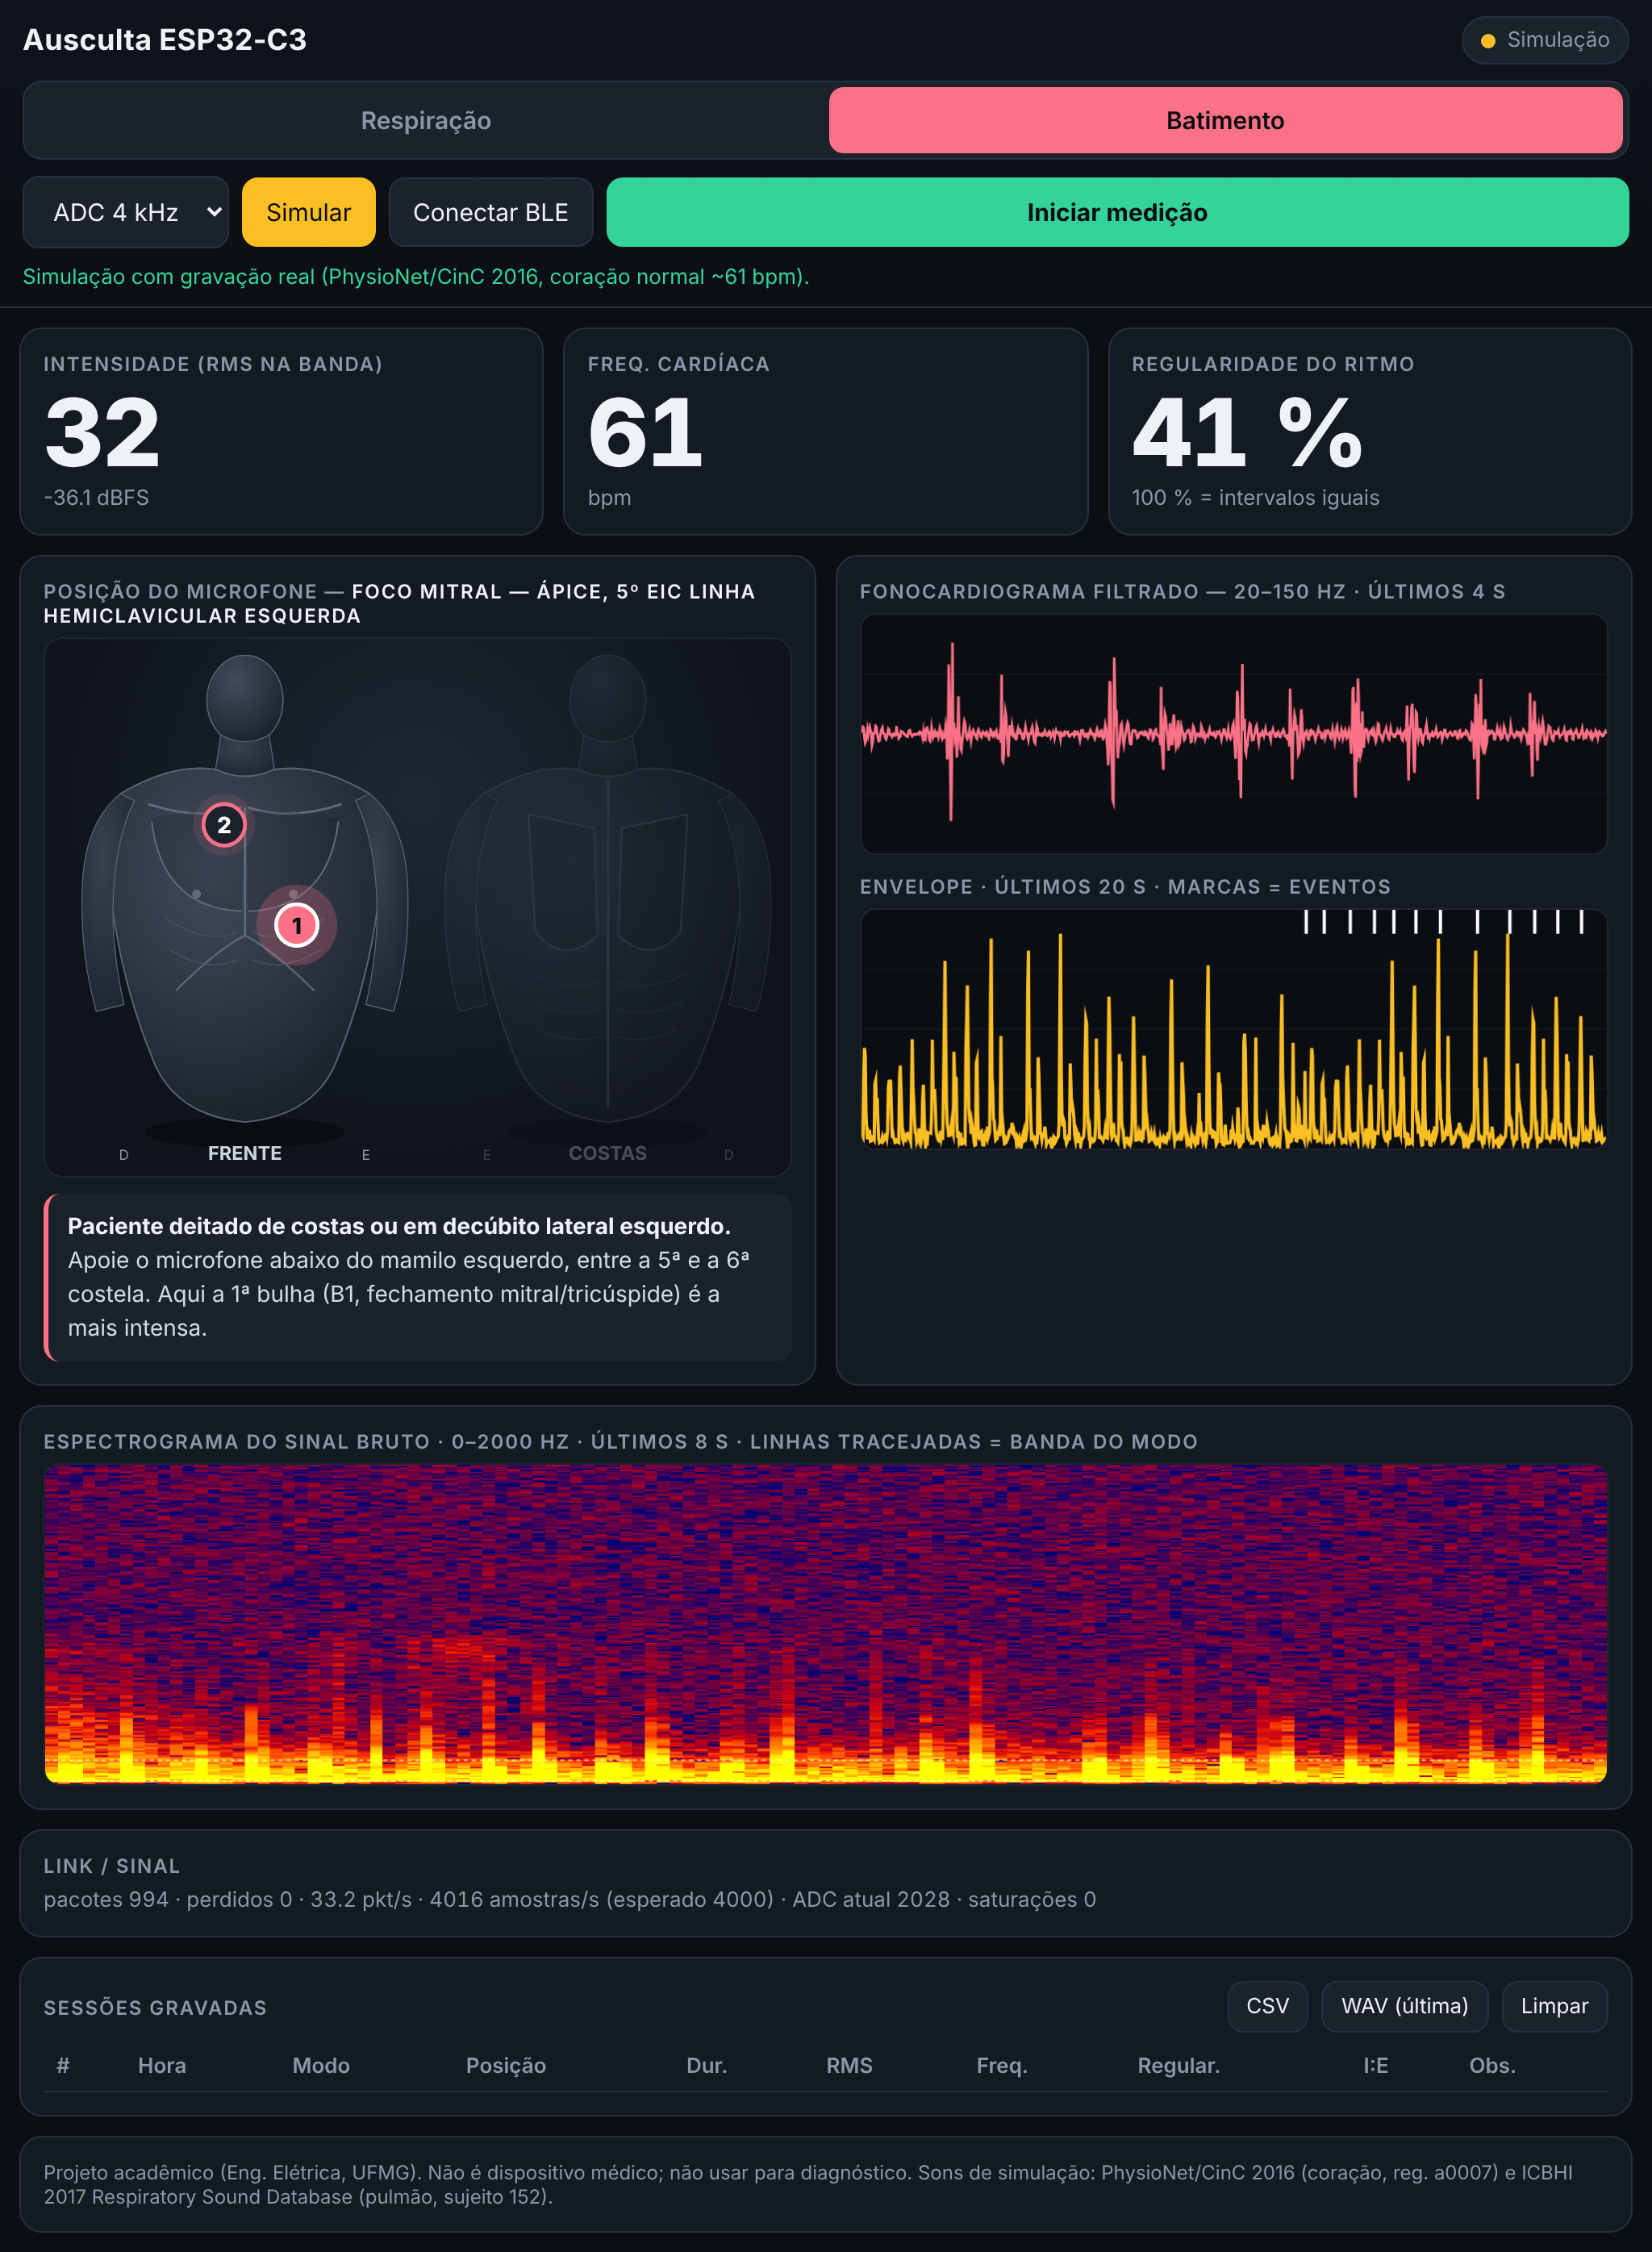
\includegraphics[width=0.49\textwidth]{fig_hr.png}
\caption{Esquerda: modo \emph{Respiração}, com gravação real de pulmão saudável (ICBHI 2017, sujeito 152). Resultado esperado: 21--23~rpm, envelope com um pico largo por ciclo. Direita: modo \emph{Batimento}, com gravação real de coração normal (PhysioNet/CinC 2016, a0007). Resultado esperado: 60--61~bpm, pares B1--B2 visíveis no fonocardiograma e no envelope. Em ambos, ``Link/sinal'' deve mostrar \textasciitilde33 pkt/s, 0 perdidos, \textasciitilde4000 amostras/s e 0 saturações.}
\label{fig:resp}\label{fig:hr}
\end{figure*}

\begin{figure}[t]
\centering
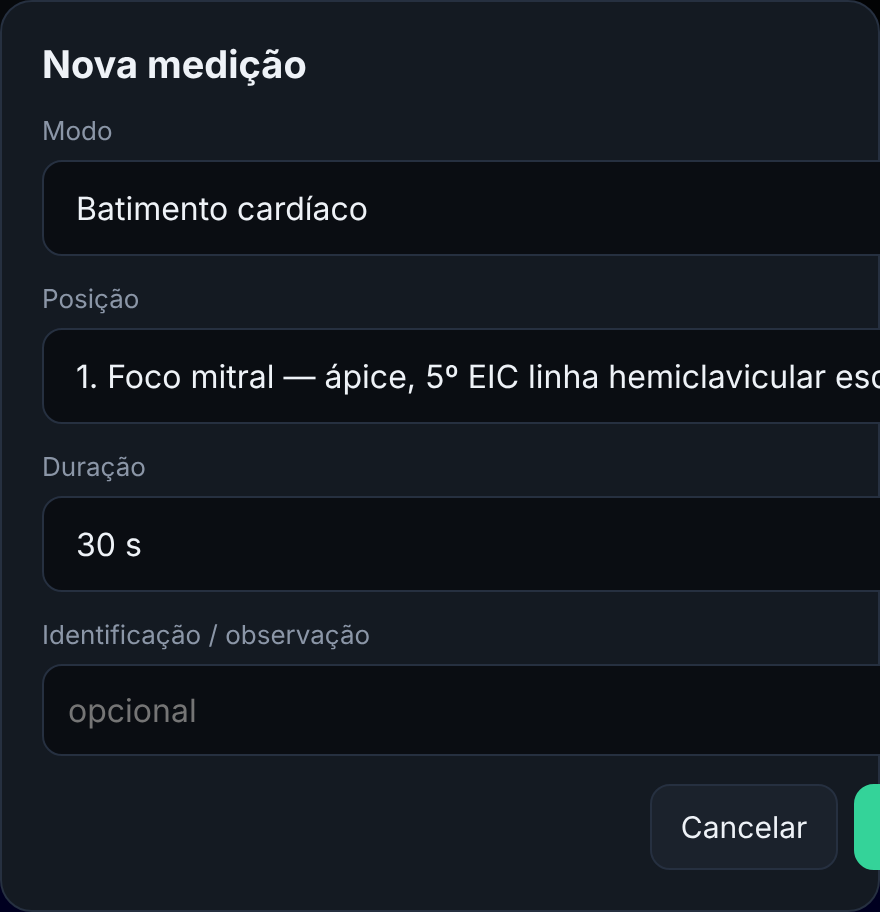
\includegraphics[width=0.75\columnwidth]{fig_dialog.png}
\caption{Pop-up ``Iniciar medição'': modo, ponto de ausculta, duração (15--120~s) e observação. Ao fim, a sessão entra na tabela com RMS médio, frequência, regularidade e I:E; CSV e WAV (sinal bruto) podem ser exportados.}
\label{fig:dlg}
\end{figure}

\subsection{Elementos comuns}
\begin{itemize}[leftmargin=*]
\item \textbf{Indicador de estado} (canto superior direito): Desconectado, Procurando, Conectado (verde), Reconectando, ou aviso amarelo quando a taxa recebida difere mais de 5\,\% da selecionada.
\item \textbf{Seletor ``ADC''}: deve ser igual à taxa do firmware (2, 4 ou 8~kHz). Os filtros e o espectrograma são recalculados.
\item \textbf{Três indicadores grandes}: intensidade RMS na banda (e em dBFS), frequência (rpm ou bpm) e um terceiro que depende do modo.
\item \textbf{Diagrama do tórax} com dois pontos por modo e, ao tocar, instrução de posicionamento do paciente e do microfone.
\item \textbf{Gráficos}: fonocardiograma filtrado (4~s), envelope (20~s, com marcas nos eventos detectados), espectrograma (8~s).
\item \textbf{Sessões}: tabela com as medições cronometradas; exportação CSV (envelope e frequência ao longo do tempo) e WAV (sinal bruto da última sessão, 16 bits, na taxa do ADC) para análise posterior em Python, MATLAB ou Audacity.
\end{itemize}

\subsection{Modo Respiração}
Banda 100--1000~Hz. Indicadores: frequência respiratória (rpm) e razão I:E (normal em repouso $\approx$1:2~\cite{bohadana2014}). Pontos: (1) frente, 2\textsuperscript{o} espaço intercostal na linha hemiclavicular direita; (2) costas, base pulmonar direita, abaixo da ponta da escápula --- o campo de maior amplitude vesicular e o mais sensível a estertores. Resultado esperado com a gravação de simulação: 21--23~rpm.

\subsection{Modo Batimento}
Banda 20--150~Hz. Indicadores: frequência cardíaca (bpm) e regularidade do ritmo (\%). Pontos: (1) foco mitral, ápice, 5\textsuperscript{o} espaço intercostal na linha hemiclavicular esquerda, onde B1 é mais intensa; (2) foco aórtico, 2\textsuperscript{o} espaço intercostal à direita do esterno, onde B2 é mais intensa. Resultado esperado com a gravação de simulação: 60--61~bpm, regularidade acima de 40\,\%.

\section{Simulação: origem dos dados e valores esperados}
\label{sec:sim}
O botão \emph{Simular} reproduz, em vez de sinal sintético, gravações reais de ausculta, já convertidas para o formato que o ADC do ESP32-C3 produzirá (4~kHz, banda 20--1000~Hz, 12 bits em torno de 2048). O objetivo é que o pipeline seja validado com sinal fisiológico de verdade antes de o hardware existir.

\begin{table}[t]
\caption{Gravações usadas na simulação}
\label{tab:sim}
\centering\small
\begin{tabularx}{\columnwidth}{@{}lYY@{}}
\toprule
 & \textbf{Coração} & \textbf{Pulmão}\\
\midrule
Base & PhysioNet/CinC Challenge 2016~\cite{liu2016,physionet} & ICBHI 2017 Respiratory Sound Database~\cite{rocha2019}\\
Registro & \code{a0007} (rótulo: normal) & \code{152\_1b1\_Al\_sc\_Meditron}\\
Sujeito & — & 16 anos, diagnóstico ``saudável'', campo anterior esquerdo, estetoscópio Meditron\\
Original & 2 kHz, 16 bit, 35,7 s & 44,1 kHz, 16 bit, 20 s\\
Usado & 12 s iniciais, reamostrados a 4 kHz & 20 s, reamostrados a 4 kHz\\
Valor de referência & 61 bpm (autocorrelação do envelope, calculada offline) & 21 rpm (7 ciclos anotados pelos autores em 20 s; sem crepitações nem sibilos)\\
Leitura do app & 60--61 bpm & 22--23 rpm\\
Licença & Dados abertos no PhysioNet (Open Data Commons Attribution)~\cite{physionet} & Disponível para pesquisa, com atribuição~\cite{rocha2019}\\
\bottomrule
\end{tabularx}
\end{table}

A Tabela~\ref{tab:sim} resume origem, referência e resultado. Os arquivos ficam em \code{sim/} no repositório; a reamostragem e a limitação de banda foram feitas com \code{scipy} (\code{resample\_poly} e Butterworth de 2\textsuperscript{a} ordem), com normalização a 70\,\% da escala e janelas de suavização nas extremidades para reprodução em laço. O aplicativo soma um ruído de $\pm$6 LSB para imitar o ADC.

Por que esses dados podem ser usados: o conjunto do CinC 2016 é distribuído abertamente pelo PhysioNet para avaliação de algoritmos~\cite{liu2016,physionet}; o ICBHI 2017 foi publicado para o desafio científico homônimo e é disponibilizado para fins de pesquisa com citação dos autores~\cite{rocha2019}. Ambos são citados no rodapé do aplicativo e no \code{README}.

\section{Por que o Bluetooth funciona assim}
\label{sec:ble}
\textbf{Só BLE.} O ESP32-C3 implementa Bluetooth 5 LE (e Wi-Fi 2,4~GHz); não possui Bluetooth clássico~\cite{esp32c3-ds}. A Web Bluetooth, por sua vez, só fala BLE/GATT~\cite{chrome-wb}. Os dois lados coincidem.

\textbf{Papéis.} O ESP32-C3 é o \emph{periférico}: anuncia um serviço GATT e envia notificações. O navegador é a \emph{central}: ao toque no botão, chama \code{requestDevice} com filtro pelo UUID do serviço (e, como alternativa, pelo prefixo de nome ``Ausculta''); o sistema mostra o seletor de dispositivos; após a escolha, o aplicativo conecta, obtém a característica \code{DATA} e ativa as notificações~\cite{chrome-wb}.

\textbf{Advertising.} O filtro por serviço exige que o UUID de 128 bits esteja no pacote de anúncio. Como UUID (18 bytes com cabeçalho) e nome não cabem juntos nos 31 bytes do anúncio, o firmware coloca o nome no \emph{scan response}; o aplicativo filtra por qualquer dos dois.

\textbf{Vazão.} 4000 amostras/s $\times$ 2 bytes $=$ 8~kB/s $=$ 64~kbit/s. Com MTU ATT de 247 bytes, cada notificação leva até 244 bytes de carga útil; o pacote do projeto usa 242 (2 de sequência + 120 amostras), o que dá $\approx$33 notificações/s. O firmware pede intervalo de conexão de 7,5--15~ms; a 15~ms isso significa cerca de uma notificação a cada dois eventos de conexão, com folga. O Android negocia o MTU automaticamente ao conectar a partir do Chrome.

\textbf{Perdas e robustez.} O contador de sequência avança a cada pacote, enviado ou não; o aplicativo contabiliza lacunas como ``perdidos''. Ao cair a conexão, o aplicativo tenta reconectar quatro vezes com intervalos crescentes. Durante uma medição, o aplicativo mantém a tela ligada (Screen Wake Lock) para que o Android não suspenda a página.

\section{Especificação para o firmware do ESP32-C3}
\label{sec:esp}
Esta seção é autocontida, para o colega responsável pelo firmware. O arquivo \code{firmware/esp32c3\_ausculta.ino} do repositório implementa tudo o que segue (Arduino + NimBLE-Arduino) e pode ser usado como está, ajustando o pino do ADC e integrando LED e bateria. Se preferir ESP-IDF, a Tabela~\ref{tab:esp} é o contrato; o aplicativo não precisa mudar.

\begin{table}[t]
\caption{Contrato de interface ESP32-C3 $\leftrightarrow$ aplicativo}
\label{tab:esp}
\centering\footnotesize
\begin{tabularx}{\columnwidth}{@{}>{\bfseries}p{1.75cm}p{3.1cm}Y@{}}
\toprule
Parâmetro & Valor & Motivo / fonte\\
\midrule
Taxa de amostragem & 4000 Hz, período fixo (250 µs) & Banda analógica até 1 kHz; $\geq$2,5$\times$ evita \emph{aliasing}. Deve ser igual ao menu ``ADC'' do app.\\
Resolução & 12 bits, valor cru 0--4095 & ADC SAR nativo do C3~\cite{esp32c3-ds}.\\
Unidade/pino & Somente ADC1: GPIO0--GPIO4 & ADC2 (GPIO5) não é suportado em modo \emph{oneshot} no C3 por limitação de hardware (errata); resultados instáveis~\cite{idf-adc}.\\
Atenuação & 12 dB (\code{ADC\_11db} no Arduino) & Faixa mensurável 0--2500 mV no C3~\cite{idf-adc}. Polarizar o sinal em $\approx$1,25 V.\\
BLE & Servidor GATT. Serviço \code{0000ff00-0000-1000-}\allowbreak\code{8000-00805f9b34fb}; característica \code{0000ff01-0000-1000-}\allowbreak\code{8000-00805f9b34fb}, propriedade NOTIFY & O app conecta por esse UUID.\\
Pacote & \code{seq} (uint16 LE) + 120 $\times$ uint16 LE $=$ 242 bytes & Cabe em MTU 247 $-$ 3; $\approx$33 pacotes/s.\\
MTU & 247 (\code{setMTU(247)}) & Vazão de 64 kbit/s.\\
Intervalo de conexão & 7,5--15 ms, latência 0, timeout 2 s & Pedido pelo periférico em \code{onConnect}.\\
Advertising & UUID do serviço no pacote principal; nome \code{Ausculta-C3} no \emph{scan response} & Não cabem juntos em 31 bytes.\\
\code{seq} & Incrementa sempre, inclusive sem conexão & O app mede perdas pela lacuna.\\
No ESP & Nada além disso & Sem filtro, sem RMS, sem modo.\\
\bottomrule
\end{tabularx}
\end{table}

\subsection{Cuidados de implementação}
\begin{enumerate}[leftmargin=*]
\item Não chamar \code{analogRead} dentro de ISR de timer no Arduino-ESP32; a temporização por \code{micros()} no \code{loop()} é suficiente. A opção mais elegante é o driver \code{adc\_continuous} (DMA) do ESP-IDF.
\item Nenhum \code{delay()} ou \code{Serial.print} no caminho de amostragem: qualquer atraso acima de 250~µs derruba a taxa, e o aplicativo acusa em ``amostras/s''.
\item LED e leitura de bateria fora do laço crítico (por exemplo, a cada $N$ pacotes).
\item Polarização e limites elétricos: sinal centrado em $\approx$1,25~V, nunca fora de 0--2,5~V. O campo ``saturações'' do aplicativo deve permanecer em zero; se subir, reduzir o ganho.
\end{enumerate}

\subsection{Teste de bancada sem microfone}
\begin{itemize}[leftmargin=*]
\item Pino do ADC em divisor resistivo de 1,25~V: ``ADC atual'' $\approx$ 2048, RMS próximo de zero, ``amostras/s'' $\approx$ 4000, ``perdidos'' 0.
\item Gerador de funções, senoide de 100~Hz e 200~mV\textsubscript{pp} sobre a polarização: linha horizontal em 100~Hz no espectrograma; RMS estável.
\item Com o microfone: tocar o diafragma deve saturar momentaneamente (contador ``saturações'' sobe) e voltar a zero em repouso.
\end{itemize}

\section{Operação: online, offline e em que aparelhos}
\label{sec:oper}
\begin{itemize}[leftmargin=*]
\item \textbf{Primeira abertura}: requer internet, para baixar a página de \url{https://daviazvd.github.io/estetoscopio-esp32/} (HTTPS, exigido pela Web Bluetooth~\cite{mdn-wb}).
\item \textbf{Depois}: funciona \emph{offline}. O \emph{service worker} guarda a página, o manifesto e as gravações de simulação em cache; o Bluetooth não usa internet. Alterações publicadas são baixadas na próxima abertura com rede.
\item \textbf{Telefone de qualquer pessoa}: sim, desde que seja Android com Chrome (ou Edge/Opera/Samsung Internet) e Bluetooth LE; não há conta, instalação ou pareamento prévio. Na primeira conexão o Android pede permissão de Bluetooth e, em versões antigas, de localização (requisito do sistema para busca BLE). Não funciona em iPhone/iPad nem no Firefox~\cite{mdn-wb}.
\item \textbf{Vários aparelhos}: o ESP32-C3 aceita uma central por vez; dois telefones não podem ouvir simultaneamente.
\item \textbf{Dados}: nada sai do aparelho; não há servidor. As sessões ficam na memória da página até exportação (CSV/WAV) e são perdidas ao recarregar.
\end{itemize}

\section{Pontos em aberto e não definidos}
\label{sec:aberto}
\begin{enumerate}[leftmargin=*]
\item \textbf{Validação com hardware real.} Tudo foi testado com gravações; o enlace BLE real (vazão, perdas, alcance, consumo) ainda não foi medido. Primeiro teste: Seção~\ref{sec:esp}, bancada.
\item \textbf{Frequência de corte real dos filtros analógicos.} Assumiu-se 20--1000~Hz. Se o passa-alta estiver em 100~Hz, o modo Batimento perde B1/B2 (energia abaixo de 150~Hz~\cite{arnott1984}) e a decisão precisa ser revista.
\item \textbf{Taxa de amostragem definitiva}: 4~kHz é a recomendação; 8~kHz também é suportado pelo aplicativo (128~kbit/s, viável mas com menos margem no BLE). Decidir após medir a vazão real.
\item \textbf{Razão I:E} é uma aproximação por limiar de intensidade, não o método clínico (fluxo). Com o sinal real pode precisar de ajuste de limiar ou ser removida.
\item \textbf{Detector respiratório}: pressupõe inspiração mais audível que expiração (padrão vesicular). Em outros padrões pode contar meio ciclo a mais ou a menos. Refratário de 2,5~s limita a leitura a $\leq$24~rpm.
\item \textbf{Ganho e polarização analógicos} ainda não dimensionados para o ADC (0--2,5~V); definir com o circuito final.
\item \textbf{Bateria e consumo}: fora do escopo do aplicativo; o firmware pode no futuro enviar o nível de bateria (sugestão: uma segunda característica READ, 1 byte em \%), e o aplicativo o exibiria.
\item \textbf{Posições de ausculta}: reduzidas a duas por modo por decisão de escopo; a lista completa (focos aórtico, pulmonar, Erb, tricúspide, mitral; campos pulmonares anterior/posterior pareados) pode voltar se o trabalho exigir.
\item \textbf{Persistência}: as sessões não sobrevivem ao recarregamento da página. Se for necessário histórico, implementar armazenamento local (IndexedDB).
\item \textbf{Modelo 3D}: o diagrama é um manequim vetorial; um modelo 3D (three.js) é possível, ao custo de \textasciitilde600~kB e desempenho no tablet.
\end{enumerate}

\begin{thebibliography}{9}\small
\bibitem{chrome-wb} F. Beaufort, ``Communicating with Bluetooth devices over JavaScript,'' Chrome for Developers. [Online]. Disponível: \url{https://developer.chrome.com/docs/capabilities/bluetooth}
\bibitem{mdn-wb} MDN Web Docs, ``Web Bluetooth API'' (compatibilidade de navegadores; contexto seguro). [Online]. Disponível: \url{https://developer.mozilla.org/en-US/docs/Web/API/Web_Bluetooth_API}
\bibitem{gh-pages-https} GitHub Docs, ``Securing your GitHub Pages site with HTTPS.'' [Online]. Disponível: \url{https://docs.github.com/en/pages/getting-started-with-github-pages/securing-your-github-pages-site-with-https}
\bibitem{esp32c3-ds} Espressif Systems, \emph{ESP32-C3 Series Datasheet}, v1.7 (ou posterior): SoC RISC-V com Wi-Fi 2,4 GHz e Bluetooth 5 (LE); 2 ADCs SAR de 12 bits, até 6 canais. [Online]. Disponível: \url{https://www.espressif.com/sites/default/files/documentation/esp32-c3_datasheet_en.pdf}
\bibitem{idf-adc} Espressif Systems, ESP-IDF Programming Guide (ESP32-C3), ``Analog to Digital Converter (ADC) Oneshot Mode Driver'': ADC1 = GPIO0--4, ADC2 = GPIO5; ADC2 oneshot não suportado no C3 (errata); faixa de 0--2500 mV com atenuação 12 dB. [Online]. Disponível: \url{https://docs.espressif.com/projects/esp-idf/en/latest/esp32c3/api-reference/peripherals/adc_oneshot.html}
\bibitem{bohadana2014} A. Bohadana, G. Izbicki e S. S. Kraman, ``Fundamentals of lung auscultation,'' \emph{N. Engl. J. Med.}, vol. 370, no. 8, pp. 744--751, 2014. DOI: 10.1056/NEJMra1302901.
\bibitem{kim2023} Y. Kim \emph{et al.}, ``The coming era of a new auscultation system for analyzing respiratory sounds,'' \emph{Mil. Med. Res.}, vol. 10, art. 44, 2023 (Tabela 1: vesicular 100--1000 Hz, queda em 200 Hz). DOI: 10.1186/s40779-023-00479-3.
\bibitem{arnott1984} P. J. Arnott, G. W. Pfeiffer e M. E. Tavel, ``Spectral analysis of heart sounds: relationships between some physical characteristics and frequency spectra of first and second heart sounds in normals and hypertensives,'' \emph{J. Biomed. Eng.}, vol. 6, no. 2, pp. 121--128, 1984 (energia principal de B1 e B2 abaixo de 150 Hz).
\bibitem{liu2016} C. Liu \emph{et al.}, ``An open access database for the evaluation of heart sound algorithms,'' \emph{Physiol. Meas.}, vol. 37, no. 12, pp. 2181--2213, 2016. DOI: 10.1088/0967-3334/37/12/2181.
\bibitem{physionet} PhysioNet, ``Classification of Heart Sound Recordings: The PhysioNet/Computing in Cardiology Challenge 2016,'' v1.0.0. [Online]. Disponível: \url{https://physionet.org/content/challenge-2016/1.0.0/}
\bibitem{rocha2019} B. M. Rocha \emph{et al.}, ``An open access database for the evaluation of respiratory sound classification algorithms,'' \emph{Physiol. Meas.}, vol. 40, no. 3, art. 035001, 2019. DOI: 10.1088/1361-6579/ab03ea. Dados: \url{https://bhichallenge.med.auth.gr/}
\end{thebibliography}
\end{document}
